\chapter{Further development}
As mentioned in the introduction this project is suppose to build a fundament for more \bon{} related work on EiffelStudio. This chapter will go over some suggestions for future projects that could be in continuation of this project. This, however, is but a segment of all possible project, but this chapters purpose is to give developers an idea of what could be done.
\section{BON Extractor}
If the \bon{} extractor is to be developed further, there are a number of interesting features that could be added. 

Currently, the \bon{} extraction treats all types the same way. Every type is just mirrored into the generated \bon{} without further analysis. An interesting addition could be to analyze the inheritance of classes to see if they were of a certain kind. For example, if a class inherits from the \textsc{set} class, it is known to have the attributes of a set. The extractor could then transform the type in question into one of the predefined standard type, with the same attributes as a set. This, however, should not be forced upon the user, but rather be implemented as a feature that could be disabled at will.

In continuation of the above, if the extractor was able to recognize certain standard types it would also be able to take use of the quantifications available in the textual \bon{} language. When a feature call such as \textit{for\_all} is encountered in the EIffel source code the extractor could translate this into textual \bon{} using the \textbf{for\_all} keyword. For instance, the quantification in figure \ref{fig:agent-for-all} could be translated into textual \bon{} in figure \ref{fig:bon-for-all}.
\begin{figure}[h]
\centerline{
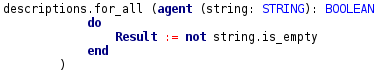
\includegraphics[scale=0.7]{images/agent_example.png} 
}
\caption{An example of an Eiffel quantification.}
\label{fig:agent-for-all}
\end{figure}

\begin{figure}[h]
\centerline{
\footnotesize{\textbf{for\_all} \textit{string} \textbf{member\_of} \textit{descriptions} \textbf{such\_that} \textit{string}:\textsc{string} \textbf{it\_holds not} \textit{string.is\_empty}}
}
\caption{How \ref{fig:agent-for-all} could be translated in textual \bon.}
\label{fig:bon-for-all}
\end{figure}
This could cause issues when agents are more advanced that in this example. In an assertion, not everything from the agent is interesting to analyze, and as such not everything should be included. The extractor could analyze what the \textit{Result} keyword relies upon and interpret that. This could easily lead to even more currently unknown complications, which is why this feature is not included in this project.

Another interesting feature to add could be the ability to switch to textual \bon{} view when viewing a cluster. In EiffelStudio the user can select a cluster and see meta about it. From this view an option to switch to both formal and informal textual \bon{} should be available. This could extract the textual \bon{} from the classes contained in the cluster, and would add to the extended overview of the code base that the \bon{} view provides.

There is no way of expressing void safety directly in \bon, only through invariants, and pre- and post-conditions. Therefore the \textit{attached} keyword does not translate to textual \bon{} in the current implementation. A possible extension could be to let the project settings from Eiffel be expressed in the extracted textual \bon{} by generating constraints for attached features. An attached feature \textit{f} could then translate into formal and informal \bon{} in the following way:
\footnotesize
\begin{verbatim}
          Invariant              Constraint
               f /= Void               "Current must have an f"
\end{verbatim}

\normalsize Last but not least, the textual \bon{} tool could be more interactive. The user could be able to add other classes from a project to a \bon{} view. Furthermore, similar to the diagram tool already in place in EiffelStudio the \bon{} tool could also work as a \textsc{case} tool. The user could add classes through the \bon{} view have them automatically translate into Eiffel source code.

\paragraph{}
Related to the \bon{} extractor it is obvious to also consider a tool working the opposite way. Generating Eiffel from textual \bon{} would allow the user to specify a full system in textual \bon{} with all features and contracts, generate the related Eiffel and he would have a full skeleton of the system. This would enable seamless interaction between specification and development.

\section{Type checker}
While the type checker on its own is quite complete, it could be improved in a number of places, especially with regards to its interaction with EiffelStudio.

First of all, it could be integrated into EiffelStudio. An ideal solution could be that whenever a piece of Eiffel source code is viewed in either the informal \bon{} view or the formal \bon{} view, the ''Compile'' button in the project bar of the EiffelStudio interface is replaced with a ''Type check'' button, running the type checker on the specification in the view. Alternatively, such a button could be placed alongside the ''Compile'' button, such that Eiffel compilation is still available from inside the \bon{} view. This would require adding a corresponding menu item to the project bar, and hooking the type checking functionality into the command executed by the button.

\paragraph{}
The current textual \bon{} specification generated by the extraction tool does not type check due to some bugs mentioned in the next section. Additionally, another fundamental aspect of extraction constitutes an obstacle for type checking. Whenever a specification is extracted, either informal or formal, the ancestors of the main class (if any) are listed in the \textit{inherit} clause of either the class chart or the class specification. But in the current implementation, only the specifications of the \emph{descendants} of the main class are extracted by the tool. As such, the main class lists ancestor classes whose specification are not found in the extracted \bon{}. Consequently, because the type checker requires that all listed ancestors are also defined in a corresponding class chart or class specification, it will complain that the ancestor classes were specified as ancestors, but never defined.

Defining the ancestors in the extracted specification is a recursive problem. Thus, if an ancestor of the main class is defined, this ancestor will also list ancestors, which in turn will list even more ancestors. As a result, all ancestors would have to be included until the root class of the inheritance hierarchy, \textsc{any}, is reached. 
\paragraph{}
Defining all the ancestors of a class in a system as extensive as EiffelStudio is clearly not a viable solution. Accordingly, a possible place for further development would be to make the type checker compatible with the limitations of the extraction tool. This could be done by either creating a new version of the type checker based on the existing version, or by adding an EiffelStudio flag to the type checker, which for instance could make sure that ancestors of the main class are not required to be defined. In either case, there should be a clear distinction between when a type checker is checking the grammar defined in \cite{walden1995}, and when it is checking an extracted specification in EiffelStudio. In the current implementation, the former has been made in order to provide a stepping stone for further development. In other words, the implemented type checker is not tailored to EiffelStudio, but supports further development in this direction.

\section{Bugs and missing features}
\subsection{BON Extractor}
\label{bugs_bon_extractors}
The \bon{} extraction tool has a few flaws. The most notable one has to do with feature calls. At the time of writing feature calls are not translated properly into textual \bon{} from Eiffel. Only the first feature of the call chain is extracted, not any following features, nor arguments. The missing information is put in a comment if the contract has no tag. Else, a tag is put in the comment instead of the missing information. A call \textit{x} on feature \textit{y} with a parameter \textit{z} it would translate as such:
\begin{center}
\textit{y.x(z)} $\rightarrow$ \textit{y.} -\-- \textit{y.x(z)}
\end{center}

Furthermore, generics of a classes don't keep their formal name throughout the class. In a class \textsc{tuple [g, h]}, the two will be represented by a G followed by an index. In the example of the tuple, the first formal generic name, \textsc{g} will be represented as G\#1 and second formal generic name, \textsc{h} as G\#2. This is still consistent and readable, but is not ideal as it can be confusing with many generics and more importantly, it does not type check.

When analyzing inheritance the consistency of comments seem to fail. The further down into the inheritance hierarchy the tool digs, the more the comments seem to vanish. To accommodate for this features without comments are extracted by name in informal \bon. When changing the point of origin (e.g., the current class) the comment structure seems to change.

All of these bugs most likely ground in a lack of understanding the abstract Eiffel syntax, which could be solved by studying this further.

Lastly, anchored types are translated directly into textual \bon. This is not purposely done, however a future extension of the type checker and the \bon{} language could be to include anchored types.

\subsection{Type checker}
A few features are missing from the implementation of the type checker.

Primarily, notational tuning as defined on page 359 in \cite{walden1995} has not been implemented in the type checker or in the parser. However, it is still possible to use the keywords and constructs of notational tuning in a specification handed over to the type checker without getting any errors. The parser does nothing but recognize the presence of these constructs (no model object are generated), while the type checker does not check it at all. Accordingly, notational tuning can be used, but support for it is not implemented.
\paragraph{}
In terms of type checking, a few features have not been implemented. Firstly, renaming of features in formal specifications are not checked. Unlike for notational tuning, renaming is implemented in the parser, and as such, the type checker has all the prerequisites for implementing a check for renaming. Secondly, export status is not checked for calls in formal assertions. As a consequence, all features of a type are always available in assertions, even though the specification states an explicit selective export status. Like for renaming, support for implementing a check for this is present, but it has not been done. The reason for omitting these checks in the initial version of the type checker is lack of time and a realization that checking other parts of the grammar would provide support for a wider range of specifications.
%renaming
%selective export in queries 
[BUGS]